\section{Experiment and Discussion}
In this section, we will show a series of experimental results including 
a) evaluation for co-segmentation and joint registration on synthetic data in which we compare our method to previous methods  b) investigation on the robustness of our method on point completeness and amount of user interaction c) testing on one group of real data and verifying the result visually.

In the experiments, the synthetic datasets are generated as follows:
\begin{enumerate}
	\item Acquire meshes for objects from 3D Warehouse.
	\item Turn the meshes into point sets with sampling method of \cite{PossionSampling}
	\item Manually place and move the point sets of objects into different point sets of scenes.   
\end{enumerate}
The real dataset (as shown in Figure~\ref{fig:realdata}) is acquired as follows:
\begin{enumerate}
	\item Scan the scenes with method of \cite{KinectFusion} 
	\item Remove walls and floors with plane fitting
	\item Turn the meshes of scenes into point sets with sampling method of \cite{PossionSampling}
\end{enumerate}

\subsection{Evaluation for Co-segmentation on Synthetic Data}
\begin{table}
	\centering
	\caption{IOU scores on three synthetic datasets. JRCS Basic is our basic formulation. JRCS Bilateral  is our bilateral formulation with point color as feature. PointNet is the semantic segmentation of \cite{qi2016pointnet} }
	\begin{tabular}{c c c c}
		Datasets & Child Shelf & Office Desk  & Living Room  \\
		\hline
		JRCS Basic & - & - & -\\   
		JRCS Bilateral & - & - & -\\
		PointNet & - & - & -\\
	\end{tabular}
	\label{tab:seg}
\end{table}
\begin{figure}[htb]
	\centering
	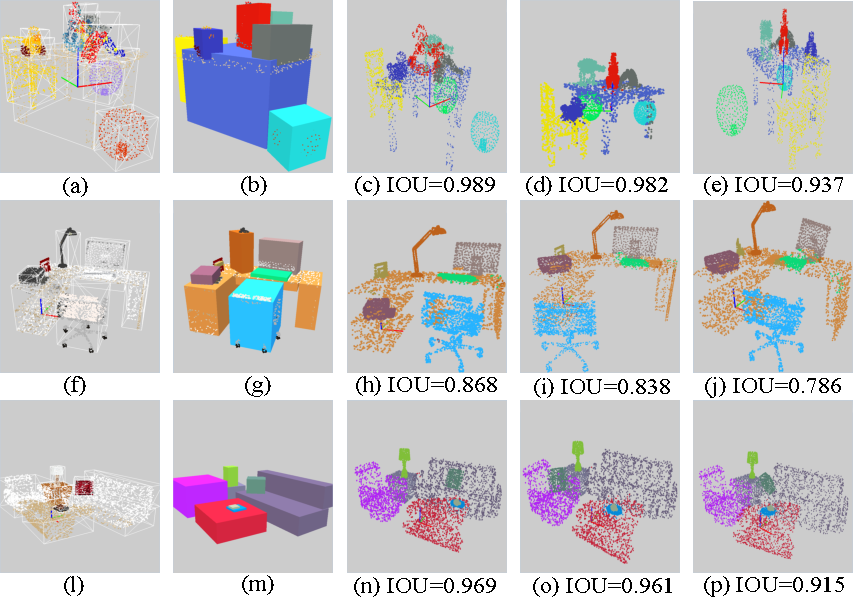
\includegraphics[width=0.8\linewidth]{images/seg/seg}
	\caption{\label{fig:seg} Segmentation evaluations on three groups of synthetic data (From top to bottom: child table, office desk, living room). Each group of data have 13 point sets. Columns from left to right: (a) Examples of point sets for each group of data. The groundtruth bounding boxes of objects in the 3D model are shown in white. (b) Manually placed boxes \cxj{on one point set}; Three segmentation results with (c) maximum IOU scores, (d) median IOU scores and (e) minimum IOU scores in the groups.}
\end{figure}
From the perspective of co-segmentation, we quantitatively evaluate our algorithm on three group of synthetic data of indoor scenes. 
%
To estimate the power of the algorithm, we only input layout for one point set in each group for initialization and do not add further interaction.
%
For numerical estimation, we calculate the intersection over union (IOU) scores for the result segmentation against ground-truth segmentation. 
In order to compare with the semantic segmentation method of PointNet\cite{qi2016pointnet}, we produce the "Living Room" with objects inside 13 object classes of PointNet\cite{qi2016pointnet}.
Table~\ref{tab:seg} shows the numeric result and Figure~\ref{fig:seg} shows some samples of visual result.
From the evaluation, we want to discuss one interesting observation:\\
%
For all three groups, the point set with highest IOU score is not the same as the point set equipped with manually placed layout.
In other words, the point sets from Figure~\ref{fig:seg}(c) are not the same point sets from Figure~\ref{fig:seg}(b). 
In the first group of data (dataset of child table in Figure~\ref{fig:seg}), the segmentation result of the point set with layout is even the second worst in the sense of IOU score. We believe this is because that the manually placed layout is not accurate respecting to point-wise segmentation. 
At early iterations of the optimization, the alteration in (\ref{equ:alteralpha}) can serve as a soft constraint to help constraining the shape of object, but in the final iterations the alteration will obstruct the further improvement of segmentation for the correspondent point set. 
\subsection{Evaluation for Joint Registration on Synthetic Data}
From the perspective of joint registration, we first compare our method with \cite{Evangelidis2014} on the synthetic point sets released by \cite{Evangelidis2014}. These data contains four point sets of Stanford Bunny with different noise and outliers. From the experiment result shown in Table~\ref{tab:reg} and Figure~\ref{fig:reg}, we can see that when dealing with one object, our method have similar result with \cite{Evangelidis2014}.
\begin{table}
	\centering
	\caption{This table shows the RMSE of joint registration on 4 point sets of Stanford Bunny. JRMPC is the method of \cite{Evangelidis2014}. JRCS Basic is our basic formulation}
	\begin{tabular}{c c c c}
		Point Sets& View 2 & View 3 & View 4 \\
		\hline
		JRMPC & 0.1604 & 0.1719 & 0.1838\\   
		JRCS Basic & 0.0822 &  0.1570  & 0.2301\\
	\end{tabular}
	\label{tab:reg}
\end{table}
\begin{figure}[htb]
	\centering
	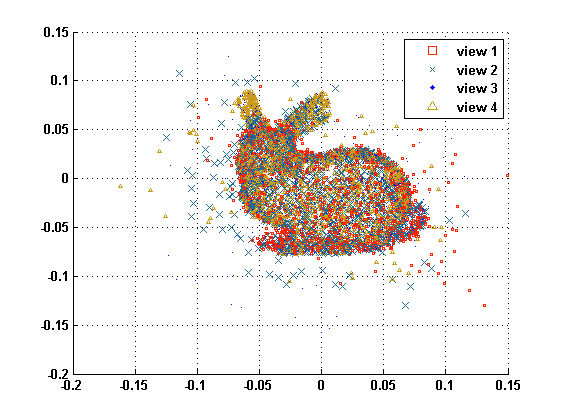
\includegraphics[width=0.4\linewidth]{images/JRMPC.png}
	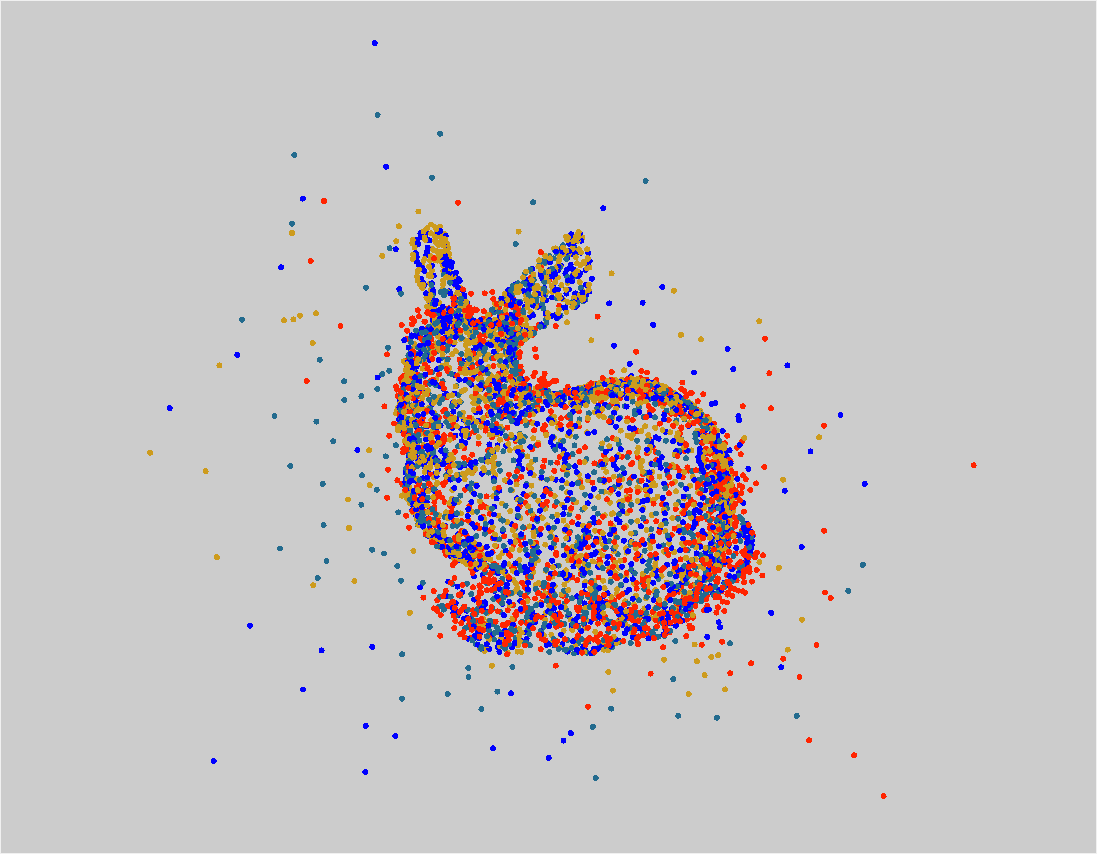
\includegraphics[width=0.4\linewidth]{images/JRCSReg.png}
	\caption{This figure shows the visual result of joint registration on 4 point sets of Stanford Bunny by JRMPC(\cite{Evangelidis2014} at left) and JRCS Basic( our basic formulation at right) }
	\label{fig:reg}
\end{figure}
We then evaluate the result by transferring the point cloud of objects to each input point set based on result $\{\phi_{mn}\}$ and calculating the average distance from a point to its true correspondent point for each input point set.
We use this average distance as fitness error to evaluate the registration quality respect to each input set.
\begin{equation}
\label{equ:error}
\vb{t}_{mn}=\frac{\sum_{\vb{v}_{mi} \in B_n}\vb{v}_{mi}}{N(B_n)}-\vb{c}_n
\end{equation}
Table~\ref{tab:regerror} shows the result of this evaluation.
\begin{table}
	\centering
	\caption{Registration errors of the three groups of synthetic data in Figure~\ref{fig:seg}. The errors are measured in meter. \cxj{3 cm is actually large error...}}
	\begin{tabular}{c c c c}
		Dataset & Maximum Error & Median Error & Minimum Error \\
		\hline
		Child Shelf & - & - & - \\   
		Office Desk & -  & - & - \\
		Living Room & -  & - & -\\
	\end{tabular}
	\label{tab:regerror}
\end{table}
For this evaluation we want to discuss that:\\
We find that even the input set with high IOU scores in segmentation can result in high fitness error. We believe this is due to the symmetric and near-symmetric objects in the scene. For symmetric objects, even the registration is correct the distance from a point to its true correspondent point can be high, since the rotation in registration result can be different from the one we use to generate this synthetic data. For near-symmetric objects, the registration often gets stuck in a local optimal and results in a high IOU score but a high fitness error.
\subsection{Investigation on Interaction}
\label{subsec:interact}
For parameter initialization and object shape constraint, we only need user to input layout (boxes) in one of the input point sets. However, our algorithm will stuck at local minimum on handling non-local motion of objects. In such challenging cases, we require more user input to further guide the optimization. In this subsection, we show an example of such challenging case and invesigate on the amount of interaction that is needed for the improvement of result. Figure~\ref{fig:interact_number} shows how the IOU score increases along with the amount of interaction.
\begin{figure}
	\centering
	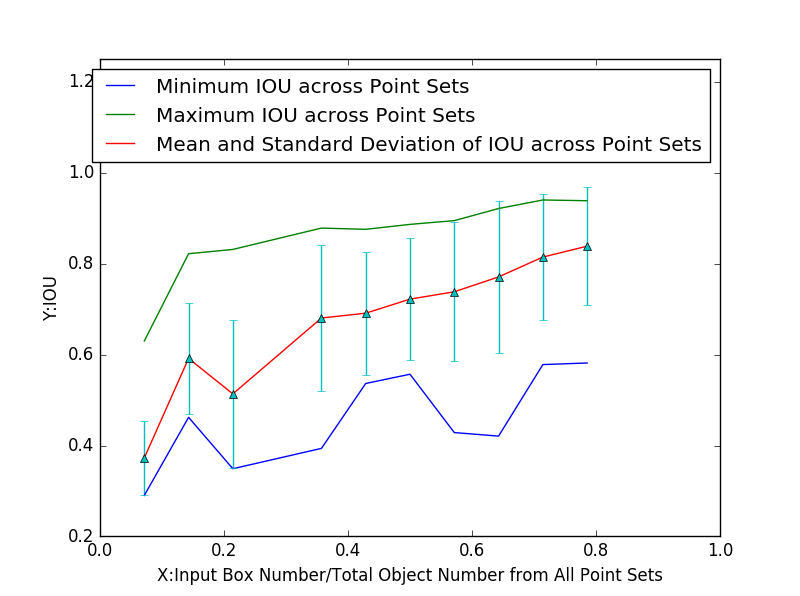
\includegraphics[width=\linewidth]{images/interact/IOU.png}
	\caption{This figure shows an example of how the amount of interaction affect the IOU score of co-segmentation,the X axis is ratio: $x=\frac{Input~Box~Number}{Total~Object~Number}$. $x=1.0$ means that the user have input one box for each object in all point sets}
	\label{fig:interact_number}
\end{figure}

\begin{figure}
	\centering
	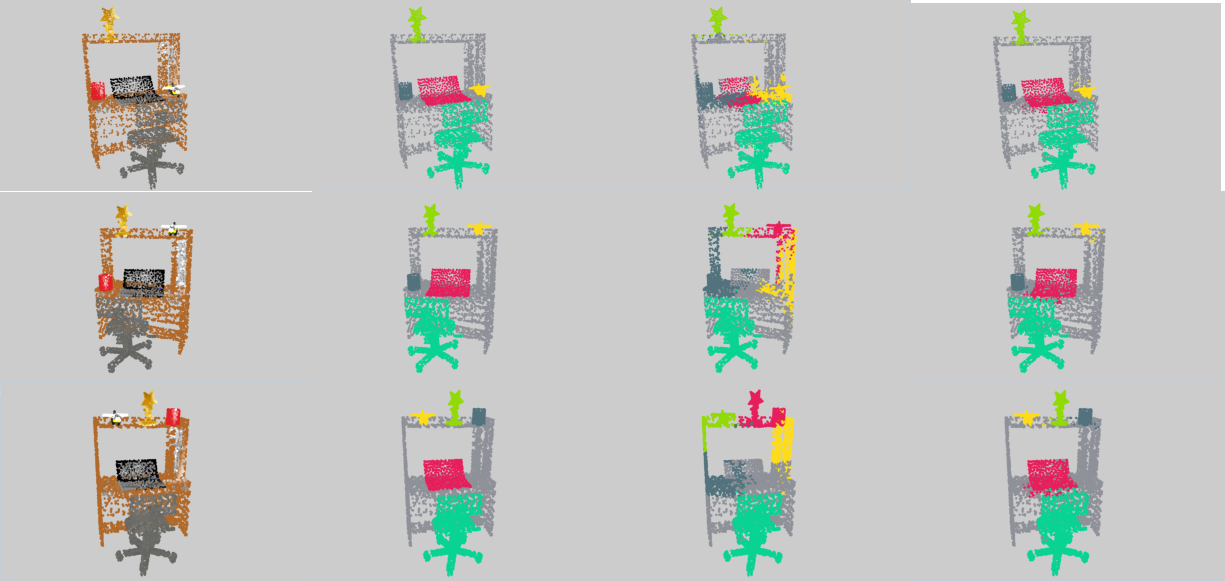
\includegraphics[width=\linewidth]{images/interact/interact}
	\caption{This figure shows 3 out of 16 point sets for experiment on amount of interaction. The first column shows the input point sets, the second column shows the groundtruth segmentation. The third column shows the visual result when 8 boxes are input. The third column shows the visual result when 88 boxes are input.}
	\label{fig:interact_vis}
\end{figure}

\subsection{Investigation on Influence of Point Incompleteness}
In previous evaluation on synthetic data, we use data that the objects are evenly and completely covered by the sampled points. In this subsection, we investigate how the point set incompleteness affect result of our algorithm. To do this, we pick a group of point sets that can converge well ( IOU $> 99\%$ for each point set ) when the point sets are complete. We then gradually remove certain percentage ( $0\%-30\%$ ) of points from each point set. The Figure~\ref{fig:incompleteness} shows how the IOU score is affected with the increasing point set incompleteness. The Figure~\ref{fig:incompleteness2} shows the visual result of this experiment. 

In order to simulate the point incompleteness caused by occlusion using a simple method, we generate the incomplete point sets with incompleteness of $p\%$ as follows:
\begin{enumerate}
	\item We randomly pick one point from each complete point set. 
	\item For one point set, sort all points ascendingly according to their euclidean distance to the picked point.  
	\item Remove the first $p\%$ points from the point set to generate a point set with incompleteness of $p\%$.
\end{enumerate}
In Figure~\ref{fig:incompleteness2}, the case of $p=\{0.0,14.0,30.0\}$ are shown. In row 09 of Figure~\ref{fig:incompleteness2} we can see that for some object in the scene half of the points are already removed.
\begin{figure}
	\centering
	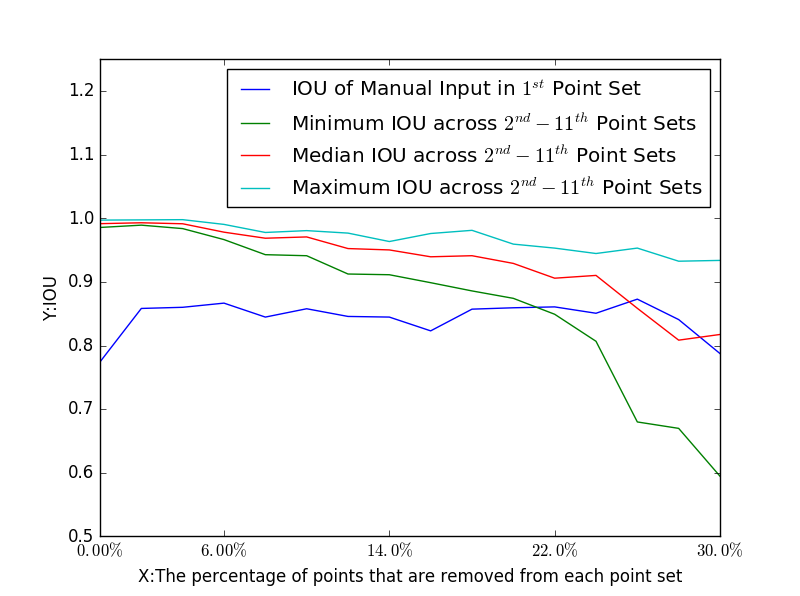
\includegraphics[width=\linewidth]{images/incompleteness/IOU.png}
	\caption{This figure shows how the data incompleteness affect the IOU score of co-segmentation}
	\label{fig:incompleteness}
\end{figure}
\begin{figure}
	\centering
	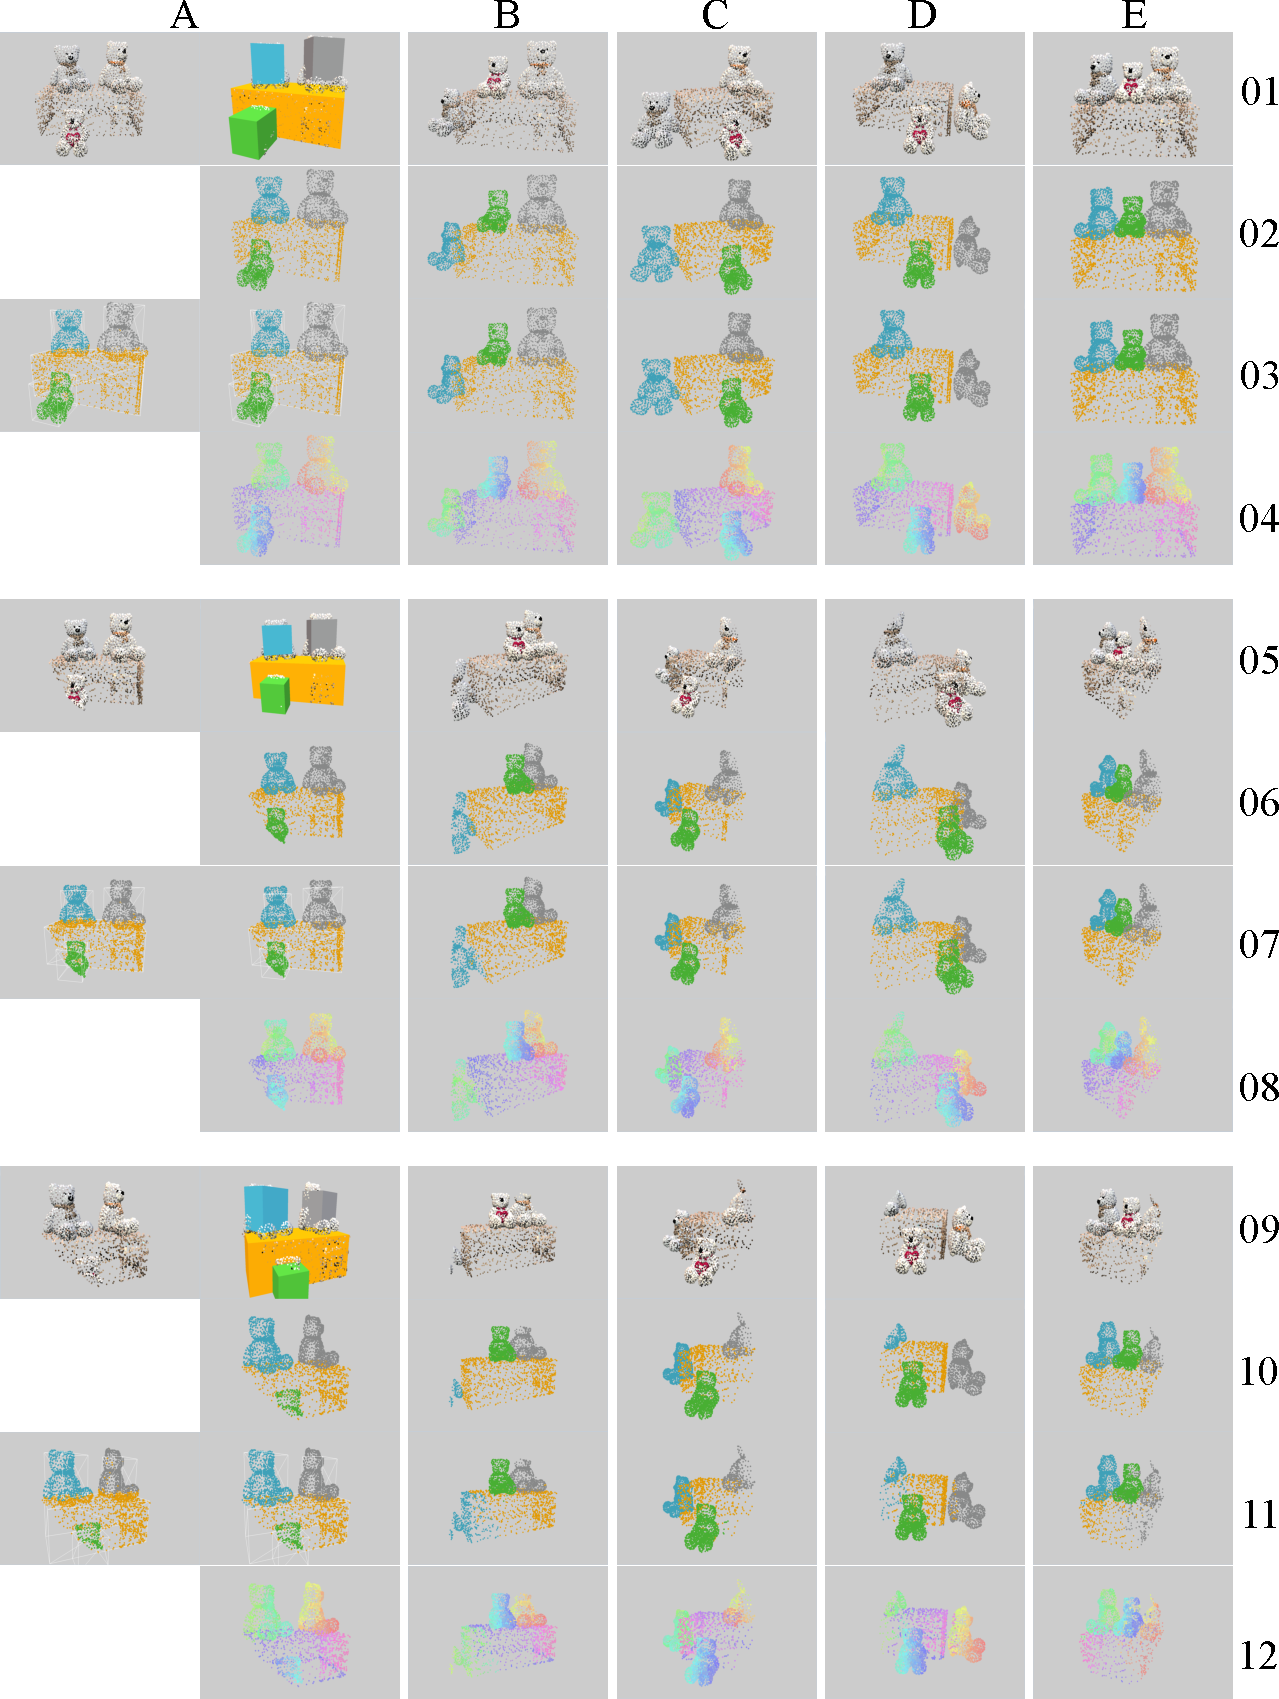
\includegraphics[width=\linewidth]{images/incompleteness/visual}
	\caption{This figure shows some of the visual result of experiments on incompleteness. This figure shows results at 3 different level of incompleteness which are $0.0\%$ at row 01-04, $14\%$ at row 05-08 and  $30\%$ at row 09-12. Each column shows the information of the same point set. Row 01,05,09 shows the inputs. For the A column the input is not only the point set but also a layout for initialization. Row 02,06,10 are ground-truth of segmentation. Row 03,04,10 are results of segmentation. For the A column, the intial segmentation and final segmentation are both shown. For the rest column, the final segmentation are shown.
	Row 04,08,12 shows the point-wise correspondences of joint registration by color-coding}
	\label{fig:incompleteness2}
\end{figure}
\subsection{Test On Real Data}
To capture real data we employ the voxel hashing method~\cite{VXH} and use plane fitting to remove walls and floors. 
We then transfer the meshes into point sets using a Poisson sampling process~\cite{PossionSampling}.
Figure~\ref{fig:challenge} shows a scanned point set. We can see that, there are noised and blurred color, shape distortion, partial scanning and outliers in real data.
%
Figure~{\ref{fig:realdata}} shows the segmentation and registration results on a group of scanned point sets.
From Figure~\ref{fig:realdata}(e), we can see that all input point sets are partitioned into objects. From the Figure~\ref{fig:realdata}(g), we can verify that the object from each input set are aligned together by the result transformation.
\begin{figure}
	\centering
	\includegraphics[width=\linewidth]{images/challenge/challenge}
	\caption{\label{fig:challenge}This figure highlights the common challenges on real data.}
\end{figure}
\begin{figure*}
	\centering
	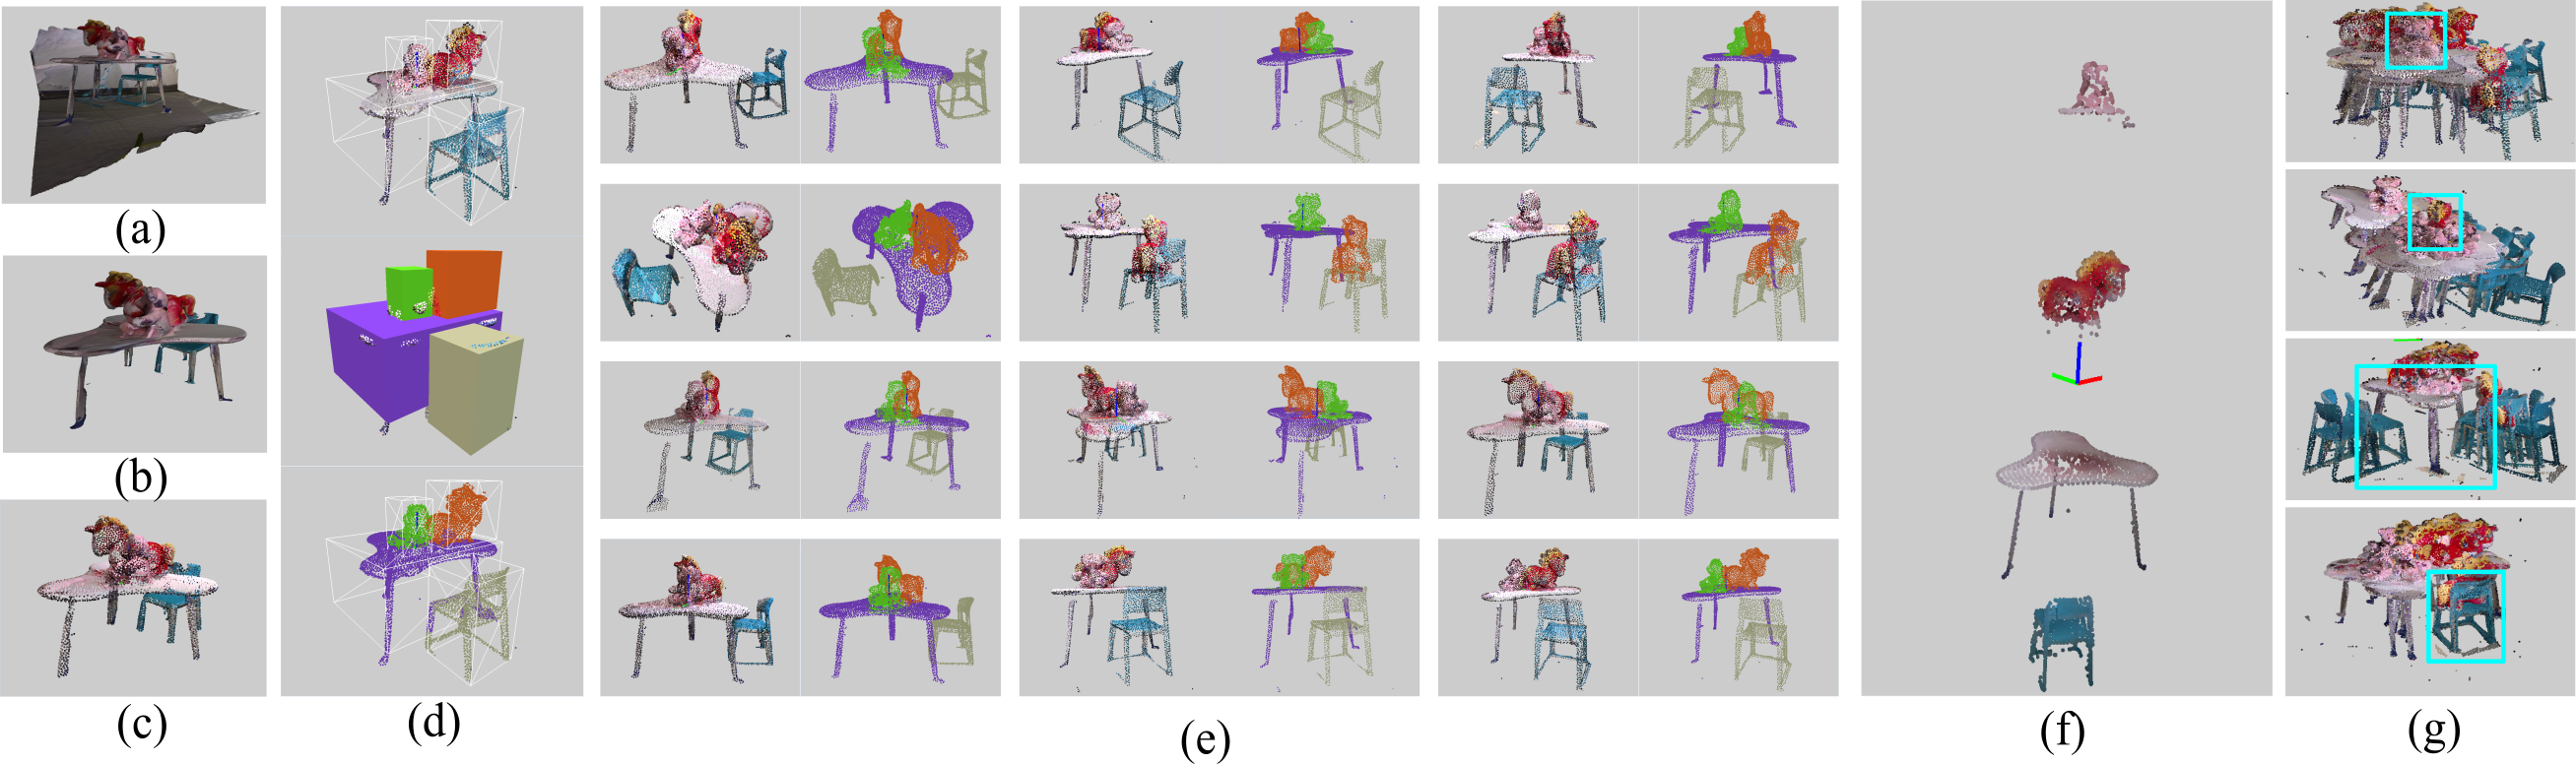
\includegraphics[width=\linewidth]{images/realdata/realdata}
	\caption{\label{fig:realdata} Segmentation and registration on real data. (a) Scanned mesh using method in \cite{VXH}. (b) Remove walls and floors by plane fitting. (c) Sampled point set using \cite{PossionSampling}. (d) With roughly placed boxes on only one point set, the points are initially segmented in this one point set. Note that parts of the chair legs are segmented to the table due to the rough box placement by users. (e) Pairs of input point sets and corresponding segmentation results. (f) The final Gaussian centroids for the five objects in the scene. (g) Verification of the registration result by aligning all point sets with respect to each object. The light blue rectangle highlights the object that is aligned together. Except the aligned object, the other objects are placed quite messy since they came from different point sets and have different arrangement relative to the aligned object. \cxj{Again, i think (g) is really messy and confusing...}  }
\end{figure*} 
\subsection{Limitations and Future Work}
\hsy{Need to add discussion on failure cases}
The biggest problem holding us back is the time performance of our current implementation.  Due to i.i.d. assumption most calculation of our algorithm can actually be parallelized. We plan to implement a new version on GPU cluster so that we can explore more potentials of our algorithm. 
For example, to integrate semantic feature vectors (generated by neural networks) into it and try it on a scene of a larger scale like \cite{GOGMA}. 
As advocated in the recent work of \cite{AGM}, it may be a good idea to do the joint registration and co-segmentation with hierarchical GMM representation when for scenes in larger scales. 